\documentclass[1p]{elsarticle_modified}
%\bibliographystyle{elsarticle-num}

%\usepackage[colorlinks]{hyperref}
%\usepackage{abbrmath_seonhwa} %\Abb, \Ascr, \Acal ,\Abf, \Afrak
\usepackage{amsfonts}
\usepackage{amssymb}
\usepackage{amsmath}
\usepackage{amsthm}
\usepackage{scalefnt}
\usepackage{amsbsy}
\usepackage{kotex}
\usepackage{caption}
\usepackage{subfig}
\usepackage{color}
\usepackage{graphicx}
\usepackage{xcolor} %% white, black, red, green, blue, cyan, magenta, yellow
\usepackage{float}
\usepackage{setspace}
\usepackage{hyperref}

\usepackage{tikz}
\usetikzlibrary{arrows}

\usepackage{multirow}
\usepackage{array} % fixed length table
\usepackage{hhline}

%%%%%%%%%%%%%%%%%%%%%
\makeatletter
\renewcommand*\env@matrix[1][\arraystretch]{%
	\edef\arraystretch{#1}%
	\hskip -\arraycolsep
	\let\@ifnextchar\new@ifnextchar
	\array{*\c@MaxMatrixCols c}}
\makeatother %https://tex.stackexchange.com/questions/14071/how-can-i-increase-the-line-spacing-in-a-matrix
%%%%%%%%%%%%%%%

\usepackage[normalem]{ulem}

\newcommand{\msout}[1]{\ifmmode\text{\sout{\ensuremath{#1}}}\else\sout{#1}\fi}
%SOURCE: \msout is \stkout macro in https://tex.stackexchange.com/questions/20609/strikeout-in-math-mode

\newcommand{\cancel}[1]{
	\ifmmode
	{\color{red}\msout{#1}}
	\else
	{\color{red}\sout{#1}}
	\fi
}

\newcommand{\add}[1]{
	{\color{blue}\uwave{#1}}
}

\newcommand{\replace}[2]{
	\ifmmode
	{\color{red}\msout{#1}}{\color{blue}\uwave{#2}}
	\else
	{\color{red}\sout{#1}}{\color{blue}\uwave{#2}}
	\fi
}

\newcommand{\Sol}{\mathcal{S}} %segment
\newcommand{\D}{D} %diagram
\newcommand{\A}{\mathcal{A}} %arc


%%%%%%%%%%%%%%%%%%%%%%%%%%%%%5 test

\def\sl{\operatorname{\textup{SL}}(2,\Cbb)}
\def\psl{\operatorname{\textup{PSL}}(2,\Cbb)}
\def\quan{\mkern 1mu \triangleright \mkern 1mu}

\theoremstyle{definition}
\newtheorem{thm}{Theorem}[section]
\newtheorem{prop}[thm]{Proposition}
\newtheorem{lem}[thm]{Lemma}
\newtheorem{ques}[thm]{Question}
\newtheorem{cor}[thm]{Corollary}
\newtheorem{defn}[thm]{Definition}
\newtheorem{exam}[thm]{Example}
\newtheorem{rmk}[thm]{Remark}
\newtheorem{alg}[thm]{Algorithm}

\newcommand{\I}{\sqrt{-1}}
\begin{document}

%\begin{frontmatter}
%
%\title{Boundary parabolic representations of knots up to 8 crossings}
%
%%% Group authors per affiliation:
%\author{Yunhi Cho} 
%\address{Department of Mathematics, University of Seoul, Seoul, Korea}
%\ead{yhcho@uos.ac.kr}
%
%
%\author{Seonhwa Kim} %\fnref{s_kim}}
%\address{Center for Geometry and Physics, Institute for Basic Science, Pohang, 37673, Korea}
%\ead{ryeona17@ibs.re.kr}
%
%\author{Hyuk Kim}
%\address{Department of Mathematical Sciences, Seoul National University, Seoul 08826, Korea}
%\ead{hyukkim@snu.ac.kr}
%
%\author{Seokbeom Yoon}
%\address{Department of Mathematical Sciences, Seoul National University, Seoul, 08826,  Korea}
%\ead{sbyoon15@snu.ac.kr}
%
%\begin{abstract}
%We find all boundary parabolic representation of knots up to 8 crossings.
%
%\end{abstract}
%\begin{keyword}
%    \MSC[2010] 57M25 
%\end{keyword}
%
%\end{frontmatter}

%\linenumbers
%\tableofcontents
%
\newcommand\colored[1]{\textcolor{white}{\rule[-0.35ex]{0.8em}{1.4ex}}\kern-0.8em\color{red} #1}%
%\newcommand\colored[1]{\textcolor{white}{ #1}\kern-2.17ex	\textcolor{white}{ #1}\kern-1.81ex	\textcolor{white}{ #1}\kern-2.15ex\color{red}#1	}

{\Large $\underline{12n_{0319}~(K12n_{0319})}$}

\setlength{\tabcolsep}{10pt}
\renewcommand{\arraystretch}{1.6}
\vspace{1cm}\begin{tabular}{m{100pt}>{\centering\arraybackslash}m{274pt}}
\multirow{5}{120pt}{
	\centering
	\includegraphics[width=112pt]{../../../GIT/diagram.site/Diagrams/png/2408_12n_0319.png}\\
\ \ \ A knot diagram\footnotemark}&
\allowdisplaybreaks
\textbf{Linearized knot diagam} \\
\cline{2-2}
 &
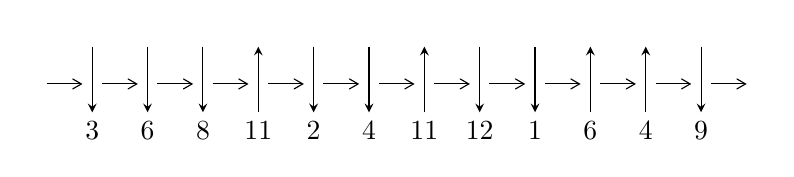
\begin{tikzpicture}[x=20pt, y=17pt]
	% nodes
	\node (C0) at (0, 0) {};
	\node (C1) at (1, 0) {};
	\node (C1U) at (1, +1) {};
	\node (C1D) at (1, -1) {3};

	\node (C2) at (2, 0) {};
	\node (C2U) at (2, +1) {};
	\node (C2D) at (2, -1) {6};

	\node (C3) at (3, 0) {};
	\node (C3U) at (3, +1) {};
	\node (C3D) at (3, -1) {8};

	\node (C4) at (4, 0) {};
	\node (C4U) at (4, +1) {};
	\node (C4D) at (4, -1) {11};

	\node (C5) at (5, 0) {};
	\node (C5U) at (5, +1) {};
	\node (C5D) at (5, -1) {2};

	\node (C6) at (6, 0) {};
	\node (C6U) at (6, +1) {};
	\node (C6D) at (6, -1) {4};

	\node (C7) at (7, 0) {};
	\node (C7U) at (7, +1) {};
	\node (C7D) at (7, -1) {11};

	\node (C8) at (8, 0) {};
	\node (C8U) at (8, +1) {};
	\node (C8D) at (8, -1) {12};

	\node (C9) at (9, 0) {};
	\node (C9U) at (9, +1) {};
	\node (C9D) at (9, -1) {1};

	\node (C10) at (10, 0) {};
	\node (C10U) at (10, +1) {};
	\node (C10D) at (10, -1) {6};

	\node (C11) at (11, 0) {};
	\node (C11U) at (11, +1) {};
	\node (C11D) at (11, -1) {4};

	\node (C12) at (12, 0) {};
	\node (C12U) at (12, +1) {};
	\node (C12D) at (12, -1) {9};
	\node (C13) at (13, 0) {};

	% arrows
	\draw[->,>={angle 60}]
	(C0) edge (C1) (C1) edge (C2) (C2) edge (C3) (C3) edge (C4) (C4) edge (C5) (C5) edge (C6) (C6) edge (C7) (C7) edge (C8) (C8) edge (C9) (C9) edge (C10) (C10) edge (C11) (C11) edge (C12) (C12) edge (C13) ;	\draw[->,>=stealth]
	(C1U) edge (C1D) (C2U) edge (C2D) (C3U) edge (C3D) (C4D) edge (C4U) (C5U) edge (C5D) (C6U) edge (C6D) (C7D) edge (C7U) (C8U) edge (C8D) (C9U) edge (C9D) (C10D) edge (C10U) (C11D) edge (C11U) (C12U) edge (C12D) ;
	\end{tikzpicture} \\
\hhline{~~} \\& 
\textbf{Solving Sequence} \\ \cline{2-2} 
 &
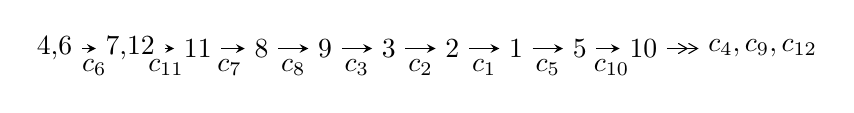
\begin{tikzpicture}[x=23pt, y=7pt]
	% node
	\node (A0) at (-1/8, 0) {4,6};
	\node (A1) at (17/16, 0) {7,12};
	\node (A2) at (17/8, 0) {11};
	\node (A3) at (25/8, 0) {8};
	\node (A4) at (33/8, 0) {9};
	\node (A5) at (41/8, 0) {3};
	\node (A6) at (49/8, 0) {2};
	\node (A7) at (57/8, 0) {1};
	\node (A8) at (65/8, 0) {5};
	\node (A9) at (73/8, 0) {10};
	\node (C1) at (1/2, -1) {$c_{6}$};
	\node (C2) at (13/8, -1) {$c_{11}$};
	\node (C3) at (21/8, -1) {$c_{7}$};
	\node (C4) at (29/8, -1) {$c_{8}$};
	\node (C5) at (37/8, -1) {$c_{3}$};
	\node (C6) at (45/8, -1) {$c_{2}$};
	\node (C7) at (53/8, -1) {$c_{1}$};
	\node (C8) at (61/8, -1) {$c_{5}$};
	\node (C9) at (69/8, -1) {$c_{10}$};
	\node (A10) at (11, 0) {$c_{4},c_{9},c_{12}$};

	% edge
	\draw[->,>=stealth]	
	(A0) edge (A1) (A1) edge (A2) (A2) edge (A3) (A3) edge (A4) (A4) edge (A5) (A5) edge (A6) (A6) edge (A7) (A7) edge (A8) (A8) edge (A9) ;
	\draw[->>,>={angle 60}]	
	(A9) edge (A10);
\end{tikzpicture} \\ 

\end{tabular} \\

\footnotetext{
The image of knot diagram is generated by the software ``\textbf{Draw programme}" developed by Andrew Bartholomew(\url{http://www.layer8.co.uk/maths/draw/index.htm\#Running-draw}), where we modified some parts for our purpose(\url{https://github.com/CATsTAILs/LinksPainter}).
}\phantom \\ \newline 
\centering \textbf{Ideals for irreducible components\footnotemark of $X_{\text{par}}$} 
 
\begin{align*}
I^u_{1}&=\langle 
2.38952\times10^{93} u^{31}-2.15372\times10^{94} u^{30}+\cdots+2.56436\times10^{95} b-7.20111\times10^{95},\\
\phantom{I^u_{1}}&\phantom{= \langle  }-8.99453\times10^{94} u^{31}+7.55251\times10^{95} u^{30}+\cdots+1.28218\times10^{96} a+7.93300\times10^{96},\\
\phantom{I^u_{1}}&\phantom{= \langle  }u^{32}-8 u^{31}+\cdots-300 u-25\rangle \\
I^u_{2}&=\langle 
-255 u^{11}-694 u^{10}+\cdots+b-720,\;-583 u^{11}-1385 u^{10}+\cdots+a-850,\\
\phantom{I^u_{2}}&\phantom{= \langle  }u^{12}+3 u^{11}- u^{10}-7 u^9+19 u^8+99 u^7+234 u^6+343 u^5+314 u^4+179 u^3+62 u^2+12 u+1\rangle \\
\\
\end{align*}
\raggedright * 2 irreducible components of $\dim_{\mathbb{C}}=0$, with total 44 representations.\\
\footnotetext{All coefficients of polynomials are rational numbers. But the coefficients are sometimes approximated in decimal forms when there is not enough margin.}
\newpage
\renewcommand{\arraystretch}{1}
\centering \section*{I. $I^u_{1}= \langle 2.39\times10^{93} u^{31}-2.15\times10^{94} u^{30}+\cdots+2.56\times10^{95} b-7.20\times10^{95},\;-8.99\times10^{94} u^{31}+7.55\times10^{95} u^{30}+\cdots+1.28\times10^{96} a+7.93\times10^{96},\;u^{32}-8 u^{31}+\cdots-300 u-25 \rangle$}
\flushleft \textbf{(i) Arc colorings}\\
\begin{tabular}{m{7pt} m{180pt} m{7pt} m{180pt} }
\flushright $a_{4}=$&$\begin{pmatrix}0\\u\end{pmatrix}$ \\
\flushright $a_{6}=$&$\begin{pmatrix}1\\0\end{pmatrix}$ \\
\flushright $a_{7}=$&$\begin{pmatrix}1\\u^2\end{pmatrix}$ \\
\flushright $a_{12}=$&$\begin{pmatrix}0.0701502 u^{31}-0.589036 u^{30}+\cdots-53.1722 u-6.18711\\-0.00931818 u^{31}+0.0839867 u^{30}+\cdots+19.4660 u+2.80815\end{pmatrix}$ \\
\flushright $a_{11}=$&$\begin{pmatrix}0.0701502 u^{31}-0.589036 u^{30}+\cdots-53.1722 u-6.18711\\0.00428886 u^{31}-0.0294728 u^{30}+\cdots+12.8694 u+2.11228\end{pmatrix}$ \\
\flushright $a_{8}=$&$\begin{pmatrix}0.139715 u^{31}-1.09759 u^{30}+\cdots-162.772 u-15.3667\\-0.0410233 u^{31}+0.326903 u^{30}+\cdots+50.9224 u+5.87488\end{pmatrix}$ \\
\flushright $a_{9}=$&$\begin{pmatrix}-0.114284 u^{31}+0.997908 u^{30}+\cdots-72.2217 u-7.58056\\0.0357130 u^{31}-0.298486 u^{30}+\cdots-4.59855 u+0.151481\end{pmatrix}$ \\
\flushright $a_{3}=$&$\begin{pmatrix}0.00605923 u^{31}-0.0127608 u^{30}+\cdots-57.1169 u-6.41631\\0.00341044 u^{31}-0.0414358 u^{30}+\cdots+35.9729 u+4.57856\end{pmatrix}$ \\
\flushright $a_{2}=$&$\begin{pmatrix}0.00946966 u^{31}-0.0541966 u^{30}+\cdots-21.1440 u-1.83775\\0.00341044 u^{31}-0.0414358 u^{30}+\cdots+35.9729 u+4.57856\end{pmatrix}$ \\
\flushright $a_{1}=$&$\begin{pmatrix}0.102606 u^{31}-0.898043 u^{30}+\cdots+90.8067 u+10.9018\\-0.0317497 u^{31}+0.264273 u^{30}+\cdots+7.01197 u+0.281882\end{pmatrix}$ \\
\flushright $a_{5}=$&$\begin{pmatrix}0.0314017 u^{31}-0.300910 u^{30}+\cdots+57.4657 u+7.12226\\-0.00733120 u^{31}+0.0774930 u^{30}+\cdots-38.6716 u-4.73528\end{pmatrix}$ \\
\flushright $a_{10}=$&$\begin{pmatrix}0.0658613 u^{31}-0.559563 u^{30}+\cdots-66.0416 u-8.29939\\0.00428886 u^{31}-0.0294728 u^{30}+\cdots+12.8694 u+2.11228\end{pmatrix}$\\&\end{tabular}
\flushleft \textbf{(ii) Obstruction class $= -1$}\\~\\
\flushleft \textbf{(iii) Cusp Shapes $= 0.253355 u^{31}-2.01113 u^{30}+\cdots-403.608 u-50.8053$}\\~\\
\newpage\renewcommand{\arraystretch}{1}
\flushleft \textbf{(iv) u-Polynomials at the component}\newline \\
\begin{tabular}{m{50pt}|m{274pt}}
Crossings & \hspace{64pt}u-Polynomials at each crossing \\
\hline $$\begin{aligned}c_{1}\end{aligned}$$&$\begin{aligned}
&u^{32}+27 u^{31}+\cdots+673 u+1
\end{aligned}$\\
\hline $$\begin{aligned}c_{2},c_{5}\end{aligned}$$&$\begin{aligned}
&u^{32}+u^{31}+\cdots-23 u+1
\end{aligned}$\\
\hline $$\begin{aligned}c_{3}\end{aligned}$$&$\begin{aligned}
&u^{32}+2 u^{31}+\cdots-42 u-19
\end{aligned}$\\
\hline $$\begin{aligned}c_{4},c_{11}\end{aligned}$$&$\begin{aligned}
&u^{32}- u^{31}+\cdots+10 u-1
\end{aligned}$\\
\hline $$\begin{aligned}c_{6}\end{aligned}$$&$\begin{aligned}
&u^{32}-8 u^{31}+\cdots-300 u-25
\end{aligned}$\\
\hline $$\begin{aligned}c_{7}\end{aligned}$$&$\begin{aligned}
&u^{32}-3 u^{31}+\cdots+1686 u+41
\end{aligned}$\\
\hline $$\begin{aligned}c_{8},c_{9},c_{12}\end{aligned}$$&$\begin{aligned}
&u^{32}+3 u^{31}+\cdots+15 u-29
\end{aligned}$\\
\hline $$\begin{aligned}c_{10}\end{aligned}$$&$\begin{aligned}
&u^{32}+3 u^{31}+\cdots-37856 u-9991
\end{aligned}$\\
\hline
\end{tabular}\\~\\
\newpage\renewcommand{\arraystretch}{1}
\flushleft \textbf{(v) Riley Polynomials at the component}\newline \\
\begin{tabular}{m{50pt}|m{274pt}}
Crossings & \hspace{64pt}Riley Polynomials at each crossing \\
\hline $$\begin{aligned}c_{1}\end{aligned}$$&$\begin{aligned}
&y^{32}-35 y^{31}+\cdots-466213 y+1
\end{aligned}$\\
\hline $$\begin{aligned}c_{2},c_{5}\end{aligned}$$&$\begin{aligned}
&y^{32}-27 y^{31}+\cdots-673 y+1
\end{aligned}$\\
\hline $$\begin{aligned}c_{3}\end{aligned}$$&$\begin{aligned}
&y^{32}-6 y^{31}+\cdots-2866 y+361
\end{aligned}$\\
\hline $$\begin{aligned}c_{4},c_{11}\end{aligned}$$&$\begin{aligned}
&y^{32}+45 y^{31}+\cdots-158 y+1
\end{aligned}$\\
\hline $$\begin{aligned}c_{6}\end{aligned}$$&$\begin{aligned}
&y^{32}-82 y^{31}+\cdots+6850 y+625
\end{aligned}$\\
\hline $$\begin{aligned}c_{7}\end{aligned}$$&$\begin{aligned}
&y^{32}+61 y^{31}+\cdots-2599876 y+1681
\end{aligned}$\\
\hline $$\begin{aligned}c_{8},c_{9},c_{12}\end{aligned}$$&$\begin{aligned}
&y^{32}-43 y^{31}+\cdots-24875 y+841
\end{aligned}$\\
\hline $$\begin{aligned}c_{10}\end{aligned}$$&$\begin{aligned}
&y^{32}+69 y^{31}+\cdots-909927994 y+99820081
\end{aligned}$\\
\hline
\end{tabular}\\~\\
\newpage\flushleft \textbf{(vi) Complex Volumes and Cusp Shapes}
$$\begin{array}{c|c|c}  
\text{Solutions to }I^u_{1}& \I (\text{vol} + \sqrt{-1}CS) & \text{Cusp shape}\\
 \hline 
\begin{aligned}
u &= -0.197289 + 0.790742 I \\
a &= -1.185250 + 0.678056 I \\
b &= \phantom{-}0.453864 - 0.396921 I\end{aligned}
 & -1.17179 - 1.02205 I & -9.29559 - 0.44678 I \\ \hline\begin{aligned}
u &= -0.197289 - 0.790742 I \\
a &= -1.185250 - 0.678056 I \\
b &= \phantom{-}0.453864 + 0.396921 I\end{aligned}
 & -1.17179 + 1.02205 I & -9.29559 + 0.44678 I \\ \hline\begin{aligned}
u &= -0.299086 + 1.150790 I \\
a &= \phantom{-}0.0080471 + 0.0961297 I \\
b &= \phantom{-}0.628217 + 0.060085 I\end{aligned}
 & \phantom{-}2.11287 + 2.53091 I & \phantom{-}5.79491 - 0.47582 I \\ \hline\begin{aligned}
u &= -0.299086 - 1.150790 I \\
a &= \phantom{-}0.0080471 - 0.0961297 I \\
b &= \phantom{-}0.628217 - 0.060085 I\end{aligned}
 & \phantom{-}2.11287 - 2.53091 I & \phantom{-}5.79491 + 0.47582 I \\ \hline\begin{aligned}
u &= \phantom{-}0.192167 + 0.775949 I \\
a &= \phantom{-}1.404300 - 0.081966 I \\
b &= \phantom{-}0.364013 - 1.054130 I\end{aligned}
 & -6.40829 + 3.07693 I & -7.10952 - 3.47095 I \\ \hline\begin{aligned}
u &= \phantom{-}0.192167 - 0.775949 I \\
a &= \phantom{-}1.404300 + 0.081966 I \\
b &= \phantom{-}0.364013 + 1.054130 I\end{aligned}
 & -6.40829 - 3.07693 I & -7.10952 + 3.47095 I \\ \hline\begin{aligned}
u &= -1.20877\phantom{ +0.000000I} \\
a &= -0.173934\phantom{ +0.000000I} \\
b &= -2.03957\phantom{ +0.000000I}\end{aligned}
 & -6.85965\phantom{ +0.000000I} & -17.0320\phantom{ +0.000000I} \\ \hline\begin{aligned}
u &= -0.727605\phantom{ +0.000000I} \\
a &= \phantom{-}1.88288\phantom{ +0.000000I} \\
b &= -0.166504\phantom{ +0.000000I}\end{aligned}
 & -7.46881\phantom{ +0.000000I} & -13.7170\phantom{ +0.000000I} \\ \hline\begin{aligned}
u &= -0.650840\phantom{ +0.000000I} \\
a &= -0.792502\phantom{ +0.000000I} \\
b &= -0.0256764\phantom{ +0.000000I}\end{aligned}
 & -1.50430\phantom{ +0.000000I} & -6.06880\phantom{ +0.000000I} \\ \hline\begin{aligned}
u &= -0.303065 + 0.488280 I \\
a &= -1.67068 + 0.64751 I \\
b &= -1.052950 - 0.482581 I\end{aligned}
 & -1.17553 + 2.30017 I & -10.81580 - 3.72452 I\\
 \hline 
 \end{array}$$\newpage$$\begin{array}{c|c|c}  
\text{Solutions to }I^u_{1}& \I (\text{vol} + \sqrt{-1}CS) & \text{Cusp shape}\\
 \hline 
\begin{aligned}
u &= -0.303065 - 0.488280 I \\
a &= -1.67068 - 0.64751 I \\
b &= -1.052950 + 0.482581 I\end{aligned}
 & -1.17553 - 2.30017 I & -10.81580 + 3.72452 I \\ \hline\begin{aligned}
u &= \phantom{-}0.350721\phantom{ +0.000000I} \\
a &= \phantom{-}1.62466\phantom{ +0.000000I} \\
b &= -0.817925\phantom{ +0.000000I}\end{aligned}
 & -2.83439\phantom{ +0.000000I} & \phantom{-}1.03330\phantom{ +0.000000I} \\ \hline\begin{aligned}
u &= -0.089144 + 0.338495 I \\
a &= -2.77884 + 3.13257 I \\
b &= -0.124470 - 1.064190 I\end{aligned}
 & -11.30980 + 7.23064 I & -10.49848 - 5.56490 I \\ \hline\begin{aligned}
u &= -0.089144 - 0.338495 I \\
a &= -2.77884 - 3.13257 I \\
b &= -0.124470 + 1.064190 I\end{aligned}
 & -11.30980 - 7.23064 I & -10.49848 + 5.56490 I \\ \hline\begin{aligned}
u &= -0.084309 + 0.271616 I \\
a &= -1.52532 + 1.43742 I \\
b &= -0.027514 + 0.487501 I\end{aligned}
 & -0.193873 + 1.035160 I & -3.30197 - 6.61105 I \\ \hline\begin{aligned}
u &= -0.084309 - 0.271616 I \\
a &= -1.52532 - 1.43742 I \\
b &= -0.027514 - 0.487501 I\end{aligned}
 & -0.193873 - 1.035160 I & -3.30197 + 6.61105 I \\ \hline\begin{aligned}
u &= -0.263547 + 0.101009 I \\
a &= -0.39229 - 3.09375 I \\
b &= -0.088766 + 1.320520 I\end{aligned}
 & -3.69901 + 3.15402 I & -10.25267 - 6.17085 I \\ \hline\begin{aligned}
u &= -0.263547 - 0.101009 I \\
a &= -0.39229 + 3.09375 I \\
b &= -0.088766 - 1.320520 I\end{aligned}
 & -3.69901 - 3.15402 I & -10.25267 + 6.17085 I \\ \hline\begin{aligned}
u &= -0.09080 + 2.11846 I \\
a &= \phantom{-}0.508788 - 0.094674 I \\
b &= \phantom{-}1.05942 + 1.08265 I\end{aligned}
 & -10.49350 + 1.26769 I & \phantom{-0.000000 } 0 \\ \hline\begin{aligned}
u &= -0.09080 - 2.11846 I \\
a &= \phantom{-}0.508788 + 0.094674 I \\
b &= \phantom{-}1.05942 - 1.08265 I\end{aligned}
 & -10.49350 - 1.26769 I & \phantom{-0.000000 } 0\\
 \hline 
 \end{array}$$\newpage$$\begin{array}{c|c|c}  
\text{Solutions to }I^u_{1}& \I (\text{vol} + \sqrt{-1}CS) & \text{Cusp shape}\\
 \hline 
\begin{aligned}
u &= \phantom{-}2.12482 + 0.01926 I \\
a &= \phantom{-}0.001205 + 0.868470 I \\
b &= -0.29154 - 1.72481 I\end{aligned}
 & -12.56270 - 0.83637 I & \phantom{-0.000000 } 0 \\ \hline\begin{aligned}
u &= \phantom{-}2.12482 - 0.01926 I \\
a &= \phantom{-}0.001205 - 0.868470 I \\
b &= -0.29154 + 1.72481 I\end{aligned}
 & -12.56270 + 0.83637 I & \phantom{-0.000000 } 0 \\ \hline\begin{aligned}
u &= -2.36872 + 0.16438 I \\
a &= \phantom{-}0.084723 - 0.669788 I \\
b &= -0.11322 + 2.10961 I\end{aligned}
 & -7.72510 - 2.29615 I & \phantom{-0.000000 } 0 \\ \hline\begin{aligned}
u &= -2.36872 - 0.16438 I \\
a &= \phantom{-}0.084723 + 0.669788 I \\
b &= -0.11322 - 2.10961 I\end{aligned}
 & -7.72510 + 2.29615 I & \phantom{-0.000000 } 0 \\ \hline\begin{aligned}
u &= \phantom{-}2.59941 + 0.20248 I \\
a &= -0.035870 - 0.679734 I \\
b &= \phantom{-}0.71473 + 2.13119 I\end{aligned}
 & \phantom{-}18.4946 - 2.1635 I & \phantom{-0.000000 } 0 \\ \hline\begin{aligned}
u &= \phantom{-}2.59941 - 0.20248 I \\
a &= -0.035870 + 0.679734 I \\
b &= \phantom{-}0.71473 - 2.13119 I\end{aligned}
 & \phantom{-}18.4946 + 2.1635 I & \phantom{-0.000000 } 0 \\ \hline\begin{aligned}
u &= -2.80747 + 0.15741 I \\
a &= \phantom{-}0.002410 - 0.627895 I \\
b &= \phantom{-}0.69377 + 2.39073 I\end{aligned}
 & -16.6434 + 4.8981 I & \phantom{-0.000000 } 0 \\ \hline\begin{aligned}
u &= -2.80747 - 0.15741 I \\
a &= \phantom{-}0.002410 + 0.627895 I \\
b &= \phantom{-}0.69377 - 2.39073 I\end{aligned}
 & -16.6434 - 4.8981 I & \phantom{-0.000000 } 0 \\ \hline\begin{aligned}
u &= \phantom{-}3.02521 + 0.40807 I \\
a &= \phantom{-}0.006648 + 0.594266 I \\
b &= \phantom{-}0.55522 - 2.49269 I\end{aligned}
 & \phantom{-}17.8060 - 11.5990 I & \phantom{-0.000000 } 0 \\ \hline\begin{aligned}
u &= \phantom{-}3.02521 - 0.40807 I \\
a &= \phantom{-}0.006648 - 0.594266 I \\
b &= \phantom{-}0.55522 + 2.49269 I\end{aligned}
 & \phantom{-}17.8060 + 11.5990 I & \phantom{-0.000000 } 0\\
 \hline 
 \end{array}$$\newpage$$\begin{array}{c|c|c}  
\text{Solutions to }I^u_{1}& \I (\text{vol} + \sqrt{-1}CS) & \text{Cusp shape}\\
 \hline 
\begin{aligned}
u &= \phantom{-}3.68008 + 0.58451 I \\
a &= \phantom{-}0.101580 + 0.427871 I \\
b &= \phantom{-}0.25407 - 2.77344 I\end{aligned}
 & -11.97980 + 5.22512 I & \phantom{-0.000000 } 0 \\ \hline\begin{aligned}
u &= \phantom{-}3.68008 - 0.58451 I \\
a &= \phantom{-}0.101580 - 0.427871 I \\
b &= \phantom{-}0.25407 + 2.77344 I\end{aligned}
 & -11.97980 - 5.22512 I & \phantom{-0.000000 } 0\\
 \hline 
 \end{array}$$\newpage\newpage\renewcommand{\arraystretch}{1}
\centering \section*{II. $I^u_{2}= \langle -255 u^{11}-694 u^{10}+\cdots+b-720,\;-583 u^{11}-1385 u^{10}+\cdots+a-850,\;u^{12}+3 u^{11}+\cdots+12 u+1 \rangle$}
\flushleft \textbf{(i) Arc colorings}\\
\begin{tabular}{m{7pt} m{180pt} m{7pt} m{180pt} }
\flushright $a_{4}=$&$\begin{pmatrix}0\\u\end{pmatrix}$ \\
\flushright $a_{6}=$&$\begin{pmatrix}1\\0\end{pmatrix}$ \\
\flushright $a_{7}=$&$\begin{pmatrix}1\\u^2\end{pmatrix}$ \\
\flushright $a_{12}=$&$\begin{pmatrix}583 u^{11}+1385 u^{10}+\cdots+9095 u+850\\255 u^{11}+694 u^{10}+\cdots+6836 u+720\end{pmatrix}$ \\
\flushright $a_{11}=$&$\begin{pmatrix}583 u^{11}+1385 u^{10}+\cdots+9095 u+850\\465 u^{11}+1211 u^{10}+\cdots+10621 u+1084\end{pmatrix}$ \\
\flushright $a_{8}=$&$\begin{pmatrix}-12 u^{11}-34 u^{10}+\cdots-515 u-70\\-256 u^{11}-640 u^{10}+\cdots-5120 u-513\end{pmatrix}$ \\
\flushright $a_{9}=$&$\begin{pmatrix}429 u^{11}+1141 u^{10}+\cdots+10869 u+1129\\u^{11}+10 u^{10}+\cdots+332 u+47\end{pmatrix}$ \\
\flushright $a_{3}=$&$\begin{pmatrix}-47 u^{11}-140 u^{10}+\cdots-1937 u-232\\- u^{11}-3 u^{10}+\cdots-62 u-11\end{pmatrix}$ \\
\flushright $a_{2}=$&$\begin{pmatrix}-48 u^{11}-143 u^{10}+\cdots-1999 u-243\\- u^{11}-3 u^{10}+\cdots-62 u-11\end{pmatrix}$ \\
\flushright $a_{1}=$&$\begin{pmatrix}382 u^{11}+1008 u^{10}+\cdots+9202 u+932\\48 u^{11}+135 u^{10}+\cdots+1679 u+197\end{pmatrix}$ \\
\flushright $a_{5}=$&$\begin{pmatrix}-195 u^{11}-538 u^{10}+\cdots-6031 u-673\\-10 u^{11}-29 u^{10}+\cdots-441 u-59\end{pmatrix}$ \\
\flushright $a_{10}=$&$\begin{pmatrix}118 u^{11}+174 u^{10}+\cdots-1526 u-234\\465 u^{11}+1211 u^{10}+\cdots+10621 u+1084\end{pmatrix}$\\&\end{tabular}
\flushleft \textbf{(ii) Obstruction class $= 1$}\\~\\
\flushleft \textbf{(iii) Cusp Shapes $= -557 u^{11}-1504 u^{10}+1049 u^9+3665 u^8-11818 u^7-51768 u^6-113824 u^5-153844 u^4-122639 u^3-56077 u^2-13659 u-1383$}\\~\\
\newpage\renewcommand{\arraystretch}{1}
\flushleft \textbf{(iv) u-Polynomials at the component}\newline \\
\begin{tabular}{m{50pt}|m{274pt}}
Crossings & \hspace{64pt}u-Polynomials at each crossing \\
\hline $$\begin{aligned}c_{1}\end{aligned}$$&$\begin{aligned}
&u^{12}-8 u^{11}+\cdots-11 u+1
\end{aligned}$\\
\hline $$\begin{aligned}c_{2}\end{aligned}$$&$\begin{aligned}
&u^{12}-4 u^{10}+u^9+8 u^8-3 u^7-11 u^6+4 u^5+10 u^4-4 u^3-5 u^2+u+1
\end{aligned}$\\
\hline $$\begin{aligned}c_{3}\end{aligned}$$&$\begin{aligned}
&u^{12}+u^{11}+3 u^{10}+2 u^9+u^8- u^7-2 u^6-5 u^5+2 u^4-2 u^3+2 u^2-1
\end{aligned}$\\
\hline $$\begin{aligned}c_{4}\end{aligned}$$&$\begin{aligned}
&u^{12}+8 u^{10}+23 u^8- u^7+26 u^6-5 u^5+5 u^4-7 u^3-6 u^2-2 u-1
\end{aligned}$\\
\hline $$\begin{aligned}c_{5}\end{aligned}$$&$\begin{aligned}
&u^{12}-4 u^{10}- u^9+8 u^8+3 u^7-11 u^6-4 u^5+10 u^4+4 u^3-5 u^2- u+1
\end{aligned}$\\
\hline $$\begin{aligned}c_{6}\end{aligned}$$&$\begin{aligned}
&u^{12}+3 u^{11}+\cdots+12 u+1
\end{aligned}$\\
\hline $$\begin{aligned}c_{7}\end{aligned}$$&$\begin{aligned}
&u^{12}+4 u^{10}+\cdots-8 u+1
\end{aligned}$\\
\hline $$\begin{aligned}c_{8},c_{9}\end{aligned}$$&$\begin{aligned}
&u^{12}+4 u^{11}+\cdots- u+1
\end{aligned}$\\
\hline $$\begin{aligned}c_{10}\end{aligned}$$&$\begin{aligned}
&u^{12}+4 u^{11}+\cdots-2 u+1
\end{aligned}$\\
\hline $$\begin{aligned}c_{11}\end{aligned}$$&$\begin{aligned}
&u^{12}+8 u^{10}+23 u^8+u^7+26 u^6+5 u^5+5 u^4+7 u^3-6 u^2+2 u-1
\end{aligned}$\\
\hline $$\begin{aligned}c_{12}\end{aligned}$$&$\begin{aligned}
&u^{12}-4 u^{11}+\cdots+u+1
\end{aligned}$\\
\hline
\end{tabular}\\~\\
\newpage\renewcommand{\arraystretch}{1}
\flushleft \textbf{(v) Riley Polynomials at the component}\newline \\
\begin{tabular}{m{50pt}|m{274pt}}
Crossings & \hspace{64pt}Riley Polynomials at each crossing \\
\hline $$\begin{aligned}c_{1}\end{aligned}$$&$\begin{aligned}
&y^{12}-12 y^{10}+\cdots-15 y+1
\end{aligned}$\\
\hline $$\begin{aligned}c_{2},c_{5}\end{aligned}$$&$\begin{aligned}
&y^{12}-8 y^{11}+\cdots-11 y+1
\end{aligned}$\\
\hline $$\begin{aligned}c_{3}\end{aligned}$$&$\begin{aligned}
&y^{12}+5 y^{11}+7 y^{10}+7 y^8+35 y^7+16 y^6-39 y^5-26 y^4+8 y^3-4 y+1
\end{aligned}$\\
\hline $$\begin{aligned}c_{4},c_{11}\end{aligned}$$&$\begin{aligned}
&y^{12}+16 y^{11}+\cdots+8 y+1
\end{aligned}$\\
\hline $$\begin{aligned}c_{6}\end{aligned}$$&$\begin{aligned}
&y^{12}-11 y^{11}+\cdots-20 y+1
\end{aligned}$\\
\hline $$\begin{aligned}c_{7}\end{aligned}$$&$\begin{aligned}
&y^{12}+8 y^{11}+\cdots-22 y+1
\end{aligned}$\\
\hline $$\begin{aligned}c_{8},c_{9},c_{12}\end{aligned}$$&$\begin{aligned}
&y^{12}-16 y^{11}+\cdots+23 y+1
\end{aligned}$\\
\hline $$\begin{aligned}c_{10}\end{aligned}$$&$\begin{aligned}
&y^{12}+4 y^{11}+\cdots-20 y+1
\end{aligned}$\\
\hline
\end{tabular}\\~\\
\newpage\flushleft \textbf{(vi) Complex Volumes and Cusp Shapes}
$$\begin{array}{c|c|c}  
\text{Solutions to }I^u_{2}& \I (\text{vol} + \sqrt{-1}CS) & \text{Cusp shape}\\
 \hline 
\begin{aligned}
u &= -0.614910\phantom{ +0.000000I} \\
a &= -0.756088\phantom{ +0.000000I} \\
b &= \phantom{-}0.764925\phantom{ +0.000000I}\end{aligned}
 & -3.38826\phantom{ +0.000000I} & -14.4840\phantom{ +0.000000I} \\ \hline\begin{aligned}
u &= -0.215601 + 1.381410 I \\
a &= \phantom{-}0.288748 - 0.106147 I \\
b &= \phantom{-}0.283384 + 0.092414 I\end{aligned}
 & \phantom{-}1.69154 + 2.70631 I & -11.02847 - 6.50238 I \\ \hline\begin{aligned}
u &= -0.215601 - 1.381410 I \\
a &= \phantom{-}0.288748 + 0.106147 I \\
b &= \phantom{-}0.283384 - 0.092414 I\end{aligned}
 & \phantom{-}1.69154 - 2.70631 I & -11.02847 + 6.50238 I \\ \hline\begin{aligned}
u &= -0.484089 + 0.123501 I \\
a &= \phantom{-}0.24097 - 1.98728 I \\
b &= -0.879338 + 0.481043 I\end{aligned}
 & -0.12267 - 1.98013 I & -3.12844 + 2.86006 I \\ \hline\begin{aligned}
u &= -0.484089 - 0.123501 I \\
a &= \phantom{-}0.24097 + 1.98728 I \\
b &= -0.879338 - 0.481043 I\end{aligned}
 & -0.12267 + 1.98013 I & -3.12844 - 2.86006 I \\ \hline\begin{aligned}
u &= -0.445198 + 0.198592 I \\
a &= -1.35255 + 2.90526 I \\
b &= \phantom{-}0.766353 - 0.473864 I\end{aligned}
 & -5.28947 - 3.09904 I & -8.62038 + 2.82123 I \\ \hline\begin{aligned}
u &= -0.445198 - 0.198592 I \\
a &= -1.35255 - 2.90526 I \\
b &= \phantom{-}0.766353 + 0.473864 I\end{aligned}
 & -5.28947 + 3.09904 I & -8.62038 - 2.82123 I \\ \hline\begin{aligned}
u &= -0.438663\phantom{ +0.000000I} \\
a &= \phantom{-}1.76179\phantom{ +0.000000I} \\
b &= \phantom{-}1.21224\phantom{ +0.000000I}\end{aligned}
 & -6.05655\phantom{ +0.000000I} & -5.50250\phantom{ +0.000000I} \\ \hline\begin{aligned}
u &= -2.04805 + 0.64643 I \\
a &= -0.276703 + 0.652409 I \\
b &= -0.25152 - 2.07706 I\end{aligned}
 & -9.00537 - 2.27031 I & -12.11846 + 2.13201 I \\ \hline\begin{aligned}
u &= -2.04805 - 0.64643 I \\
a &= -0.276703 - 0.652409 I \\
b &= -0.25152 + 2.07706 I\end{aligned}
 & -9.00537 + 2.27031 I & -12.11846 - 2.13201 I\\
 \hline 
 \end{array}$$\newpage$$\begin{array}{c|c|c}  
\text{Solutions to }I^u_{2}& \I (\text{vol} + \sqrt{-1}CS) & \text{Cusp shape}\\
 \hline 
\begin{aligned}
u &= \phantom{-}2.21973 + 1.41604 I \\
a &= -0.403311 - 0.470237 I \\
b &= -0.90746 + 1.60507 I\end{aligned}
 & -12.16040 + 3.87633 I & -12.61114 - 1.47831 I \\ \hline\begin{aligned}
u &= \phantom{-}2.21973 - 1.41604 I \\
a &= -0.403311 + 0.470237 I \\
b &= -0.90746 - 1.60507 I\end{aligned}
 & -12.16040 - 3.87633 I & -12.61114 + 1.47831 I\\
 \hline 
 \end{array}$$\newpage
\newpage\renewcommand{\arraystretch}{1}
\centering \section*{ III. u-Polynomials}
\begin{tabular}{m{50pt}|m{274pt}}
Crossings & \hspace{64pt}u-Polynomials at each crossing \\
\hline $$\begin{aligned}c_{1}\end{aligned}$$&$\begin{aligned}
&(u^{12}-8 u^{11}+\cdots-11 u+1)(u^{32}+27 u^{31}+\cdots+673 u+1)
\end{aligned}$\\
\hline $$\begin{aligned}c_{2}\end{aligned}$$&$\begin{aligned}
&(u^{12}-4 u^{10}+u^9+8 u^8-3 u^7-11 u^6+4 u^5+10 u^4-4 u^3-5 u^2+u+1)\\
&\cdot(u^{32}+u^{31}+\cdots-23 u+1)
\end{aligned}$\\
\hline $$\begin{aligned}c_{3}\end{aligned}$$&$\begin{aligned}
&(u^{12}+u^{11}+3 u^{10}+2 u^9+u^8- u^7-2 u^6-5 u^5+2 u^4-2 u^3+2 u^2-1)\\
&\cdot(u^{32}+2 u^{31}+\cdots-42 u-19)
\end{aligned}$\\
\hline $$\begin{aligned}c_{4}\end{aligned}$$&$\begin{aligned}
&(u^{12}+8 u^{10}+23 u^8- u^7+26 u^6-5 u^5+5 u^4-7 u^3-6 u^2-2 u-1)\\
&\cdot(u^{32}- u^{31}+\cdots+10 u-1)
\end{aligned}$\\
\hline $$\begin{aligned}c_{5}\end{aligned}$$&$\begin{aligned}
&(u^{12}-4 u^{10}- u^9+8 u^8+3 u^7-11 u^6-4 u^5+10 u^4+4 u^3-5 u^2- u+1)\\
&\cdot(u^{32}+u^{31}+\cdots-23 u+1)
\end{aligned}$\\
\hline $$\begin{aligned}c_{6}\end{aligned}$$&$\begin{aligned}
&(u^{12}+3 u^{11}+\cdots+12 u+1)(u^{32}-8 u^{31}+\cdots-300 u-25)
\end{aligned}$\\
\hline $$\begin{aligned}c_{7}\end{aligned}$$&$\begin{aligned}
&(u^{12}+4 u^{10}+\cdots-8 u+1)(u^{32}-3 u^{31}+\cdots+1686 u+41)
\end{aligned}$\\
\hline $$\begin{aligned}c_{8},c_{9}\end{aligned}$$&$\begin{aligned}
&(u^{12}+4 u^{11}+\cdots- u+1)(u^{32}+3 u^{31}+\cdots+15 u-29)
\end{aligned}$\\
\hline $$\begin{aligned}c_{10}\end{aligned}$$&$\begin{aligned}
&(u^{12}+4 u^{11}+\cdots-2 u+1)(u^{32}+3 u^{31}+\cdots-37856 u-9991)
\end{aligned}$\\
\hline $$\begin{aligned}c_{11}\end{aligned}$$&$\begin{aligned}
&(u^{12}+8 u^{10}+23 u^8+u^7+26 u^6+5 u^5+5 u^4+7 u^3-6 u^2+2 u-1)\\
&\cdot(u^{32}- u^{31}+\cdots+10 u-1)
\end{aligned}$\\
\hline $$\begin{aligned}c_{12}\end{aligned}$$&$\begin{aligned}
&(u^{12}-4 u^{11}+\cdots+u+1)(u^{32}+3 u^{31}+\cdots+15 u-29)
\end{aligned}$\\
\hline
\end{tabular}\newpage\renewcommand{\arraystretch}{1}
\centering \section*{ IV. Riley Polynomials}
\begin{tabular}{m{50pt}|m{274pt}}
Crossings & \hspace{64pt}Riley Polynomials at each crossing \\
\hline $$\begin{aligned}c_{1}\end{aligned}$$&$\begin{aligned}
&(y^{12}-12 y^{10}+\cdots-15 y+1)(y^{32}-35 y^{31}+\cdots-466213 y+1)
\end{aligned}$\\
\hline $$\begin{aligned}c_{2},c_{5}\end{aligned}$$&$\begin{aligned}
&(y^{12}-8 y^{11}+\cdots-11 y+1)(y^{32}-27 y^{31}+\cdots-673 y+1)
\end{aligned}$\\
\hline $$\begin{aligned}c_{3}\end{aligned}$$&$\begin{aligned}
&(y^{12}+5 y^{11}+7 y^{10}+7 y^8+35 y^7+16 y^6-39 y^5-26 y^4+8 y^3-4 y+1)\\
&\cdot(y^{32}-6 y^{31}+\cdots-2866 y+361)
\end{aligned}$\\
\hline $$\begin{aligned}c_{4},c_{11}\end{aligned}$$&$\begin{aligned}
&(y^{12}+16 y^{11}+\cdots+8 y+1)(y^{32}+45 y^{31}+\cdots-158 y+1)
\end{aligned}$\\
\hline $$\begin{aligned}c_{6}\end{aligned}$$&$\begin{aligned}
&(y^{12}-11 y^{11}+\cdots-20 y+1)(y^{32}-82 y^{31}+\cdots+6850 y+625)
\end{aligned}$\\
\hline $$\begin{aligned}c_{7}\end{aligned}$$&$\begin{aligned}
&(y^{12}+8 y^{11}+\cdots-22 y+1)(y^{32}+61 y^{31}+\cdots-2599876 y+1681)
\end{aligned}$\\
\hline $$\begin{aligned}c_{8},c_{9},c_{12}\end{aligned}$$&$\begin{aligned}
&(y^{12}-16 y^{11}+\cdots+23 y+1)(y^{32}-43 y^{31}+\cdots-24875 y+841)
\end{aligned}$\\
\hline $$\begin{aligned}c_{10}\end{aligned}$$&$\begin{aligned}
&(y^{12}+4 y^{11}+\cdots-20 y+1)\\
&\cdot(y^{32}+69 y^{31}+\cdots-909927994 y+99820081)
\end{aligned}$\\
\hline
\end{tabular}
\vskip 2pc
\end{document}